\section{Summary}



\begin{figure}
  \begin{center}
    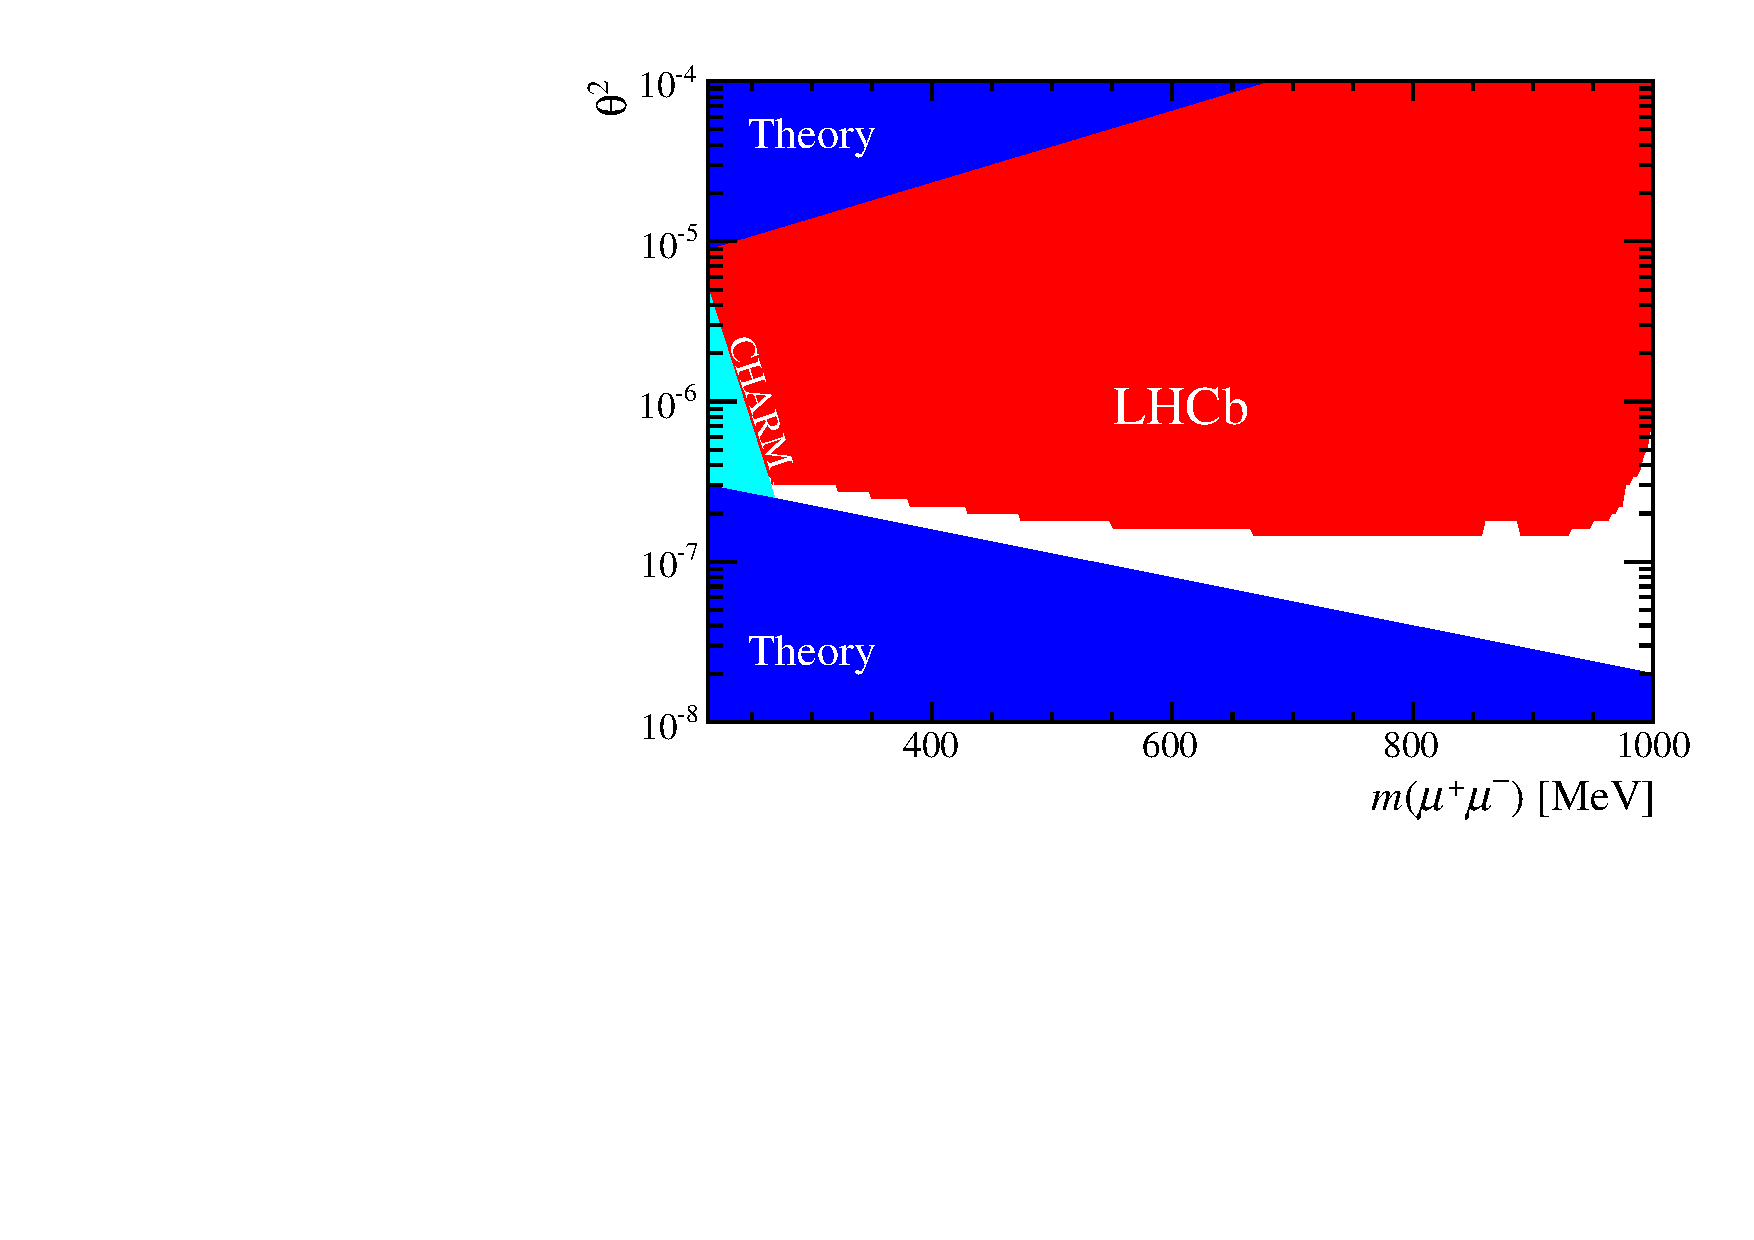
\includegraphics[width=0.48\textwidth]{kstmm_infl_excl}
    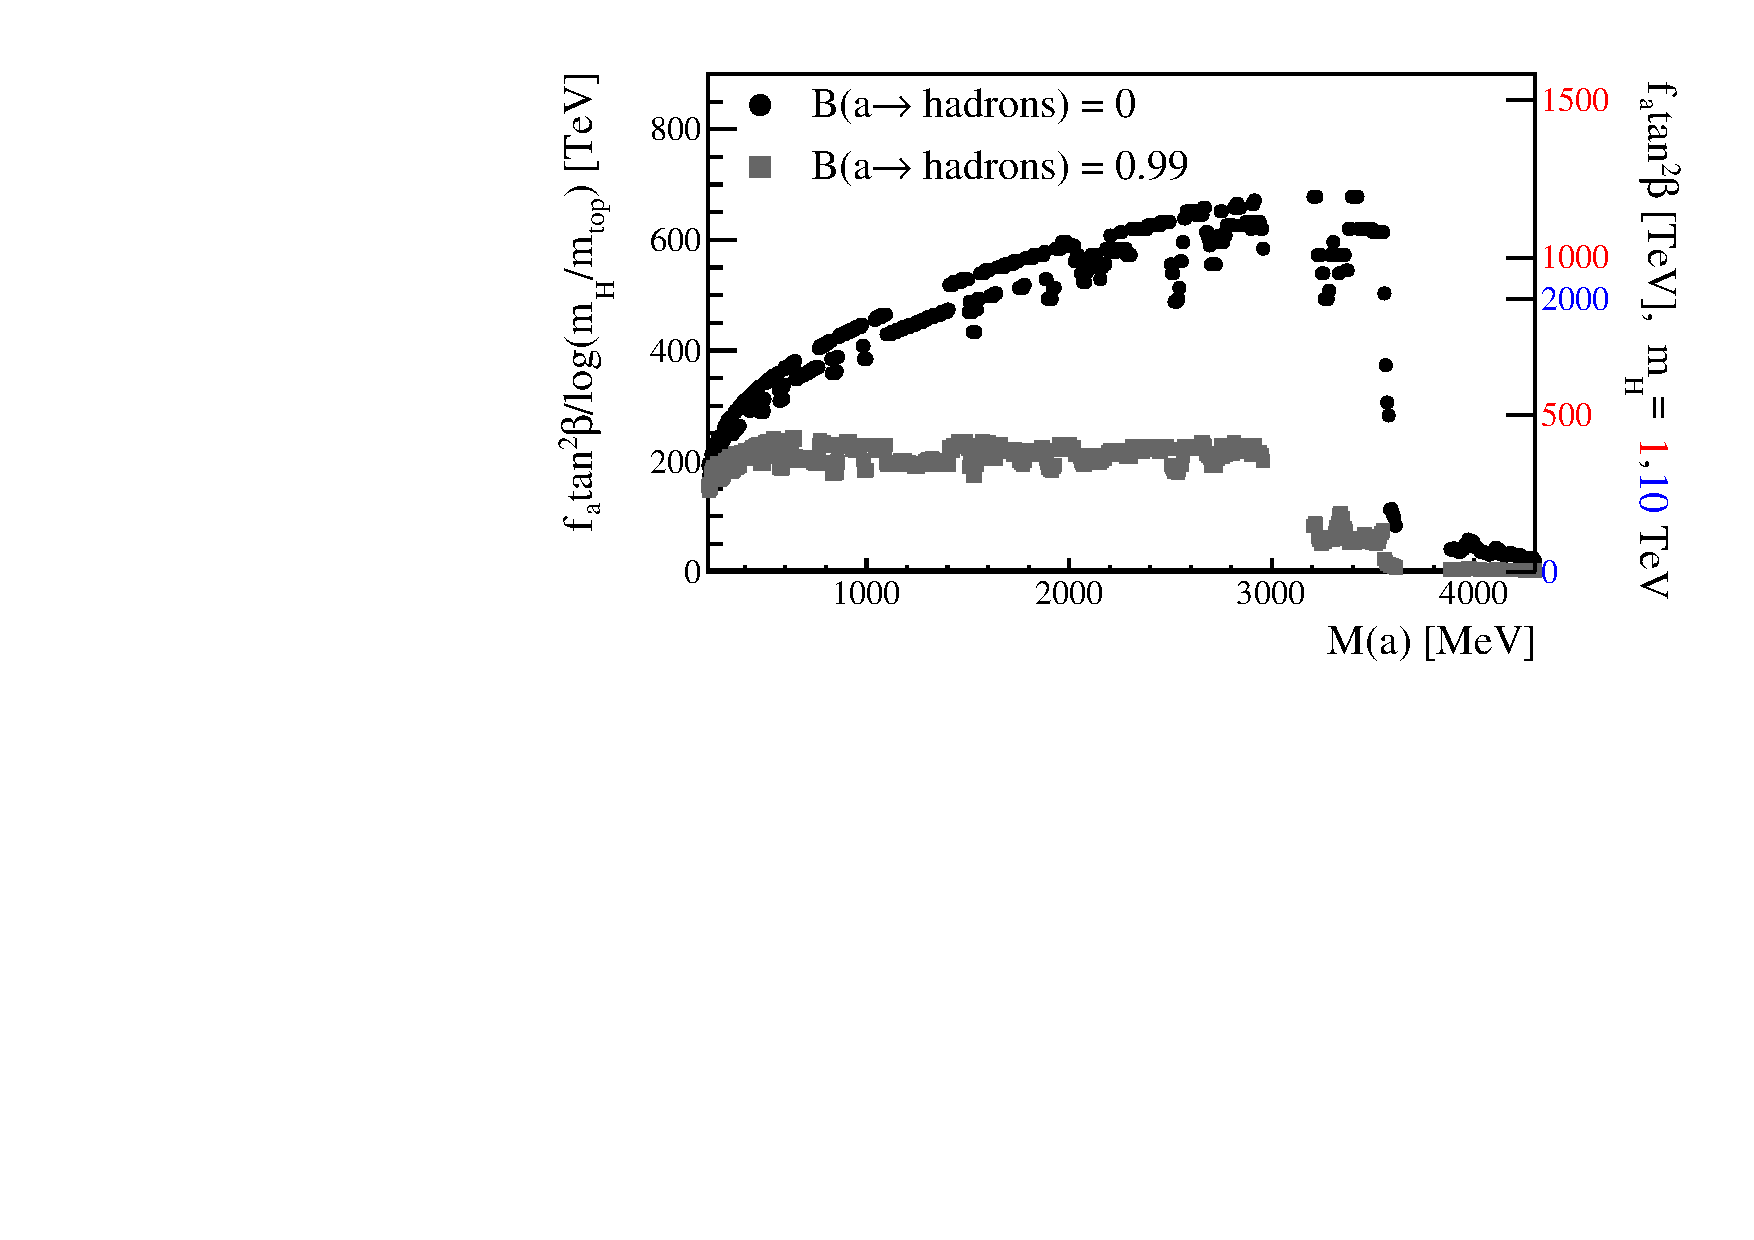
\includegraphics[width=0.48\textwidth]{kstmm_axion_excl}
    \caption[]
    {
    }
    \label{fig:db:excl}
  \end{center}
\end{figure}


%At the time of writing, this analysis is undergoing the review procedure and unblinding is ongoing.
%
%The plan is to unblind etc, and then fit if find $>3\sigma$ excess.
%
%Here, a fully frequentist method of searching for a dark boson with an unknown mass and lifetime
%has been presented.
%Specific peaking backgrounds are removed before the combinatorial background is suppressed by
%applying a \uBDT designed to yield a response which is uniform in signal efficiency in both the
%mass and lifetime dimensions.

\begin{itemize}
  \item New strategy
  \item Excellent selectio
  \item Excellent parmeterization
  \item Sensitive
\end{itemize}



